\documentclass[aspectratio=43,9pt]{beamer}
%
\usepackage{tikz}
\usepackage{enumerate}
%
\usetheme{Boadilla}
%
\graphicspath{{./figures/}}
%
\let\Tiny=\tiny%			% to avoid warnings about font size
%\usepackage{lmodern}%		% alternative method to avoid these warnings
%
\catcode`~=11 % make LaTeX treat tilde (~) like a normal character
\newcommand{\urltilde}{\hbox{~}}
\catcode`~=13 % revert back to treating tilde (~) as an active character
%
% misc commands
\newcommand{\bm}[1]{\mathbf{#1}}
\newcommand{\bs}[1]{\boldsymbol{#1}}
\newenvironment{myitemize}[1]{\vspace{#1}\begin{itemize}\setlength\itemsep{#1}}{\end{itemize}}
%
% pgf markers
\usepgflibrary{plotmarks}
%
\setbeamertemplate{footline}
{
  \leavevmode%
  \hbox{%
  \begin{beamercolorbox}[wd=.8\paperwidth,ht=2.25ex,dp=1ex,left]{author in head/foot}%
    \usebeamerfont{author in head/foot}\hspace*{4em}\inserttitle
  \end{beamercolorbox}%
  \begin{beamercolorbox}[wd=.2\paperwidth,ht=2.25ex,dp=1ex,right]{author in head/foot}%
    \usebeamerfont{author in head/foot}\insertframenumber{} / \inserttotalframenumber\hspace*{1ex}
  \end{beamercolorbox}}%
  \vskip0pt%
}
%
\setbeamertemplate{navigation symbols}{}
%
\setbeamertemplate{frametitle}
{%
	\begin{minipage}{.9\paperwidth}
		\vspace*{1ex}%
		\flushright%
		%\bfseries
		\LARGE%
		\insertframetitle%
	\end{minipage}%
}
%
\setbeamertemplate{title page}{
	\begin{center}
		\vspace*{2ex}
		\usebeamercolor[fg]{frametitle}{%
			\Large%
			Numerical Techniques 2024--2025\\[2ex]
			%
			\LARGE%
			\inserttitle
		}\\[6ex]
		\usebeamercolor[fg]{normal text}{%
			Daan Degrauwe\\[1ex]
			\texttt{daan.degrauwe@meteo.be}\\[4ex]
			Postgraduate Studies in Weather and Climate Modeling\\[1ex]
			Ghent University
		}
	\end{center}
}
%
\newcommand{\ft}[2]{{\textstyle\frac{#1}{#2}}}
%
% increase space around equations
\makeatletter
\g@addto@macro\normalsize{%
	\setlength{\abovedisplayskip}{3ex}%
	\setlength{\belowdisplayskip}{3ex}%
	\setlength{\abovedisplayshortskip}{3ex}%
	\setlength{\belowdisplayshortskip}{3ex}%
}%
\makeatother
%

%
\title{2. The oscillation equation and time differencing}%
%
%%%%%%%%%%%%%%%%%%%%%%%%%%%%%%%%%%%%%%%%%%%%%%%%%%%%%%%%%%%%%%%%%%%%%%
%
\begin{document}
%
%%%%%%%%%%%%%%%%%%%%%%%%%%%%%%%%%%%%%%%%%%%%%%%%%%%%%%%%%%%%%%%%%%%%%%%%%%%%%%%%%%%%%%%%%%%%%%%%%%%%
%
\begin{frame}[plain]
	\titlepage
\end{frame}
%
%%%%%%%%%%%%%%%%%%%%%%%%%%%%%%%%%%%%%%%%%%%%%%%%%%%%%%%%%%%%%%%%%%%%%%%%%%%%%%%%%%%%%%%%%%%%%%%%%%%%
%
\begin{frame}
	%
	\frametitle{Previously on Numerical Techniques\ldots}
	%
	\begin{itemize}
		\item Positioning of the course in the postgraduate program\vspace*{2ex}
		\item Discretization and finite differences\vspace*{2ex}
		\item Consistency, convergence and stability\vspace*{2ex}
		\item Von Neumann analysis and Courant number $\mu=c\frac{\Delta t}{\Delta x}$, linking spatial resolution to temporal resolution\vspace*{2ex}
		\item Example of upstream scheme for 1D advection equation\vspace*{2ex}
		\item Don't worry about math too much!
	\end{itemize}
	%
\end{frame}
%
%%%%%%%%%%%%%%%%%%%%%%%%%%%%%%%%%%%%%%%%%%%%%%%%%%%%%%%%%%%%%%%%%%%%%%
%
\begin{frame}
	%
	\frametitle{Today's content\ldots}
	%
	\begin{itemize}
		\item The oscillation equation\vspace*{2ex}
		\item Errors due to time discretization: amplitude and phase\vspace*{2ex}
		\item Concrete schemes\vspace*{1ex}
			\begin{itemize}
				\item Single stage, two timelevel\\
					\hspace*{5mm} Forward, backward, trapezium\vspace*{1ex}
				\item Multistage, two timelevel\\
					\hspace*{5mm} Heun, Matsuno, Runge-Kutta\vspace*{1ex}
				\item Single stage, three timelevel\\
					\hspace*{5mm} Leapfrog, Adams-Bashforth\vspace*{1ex}
				\item Filter for computational modes
			\end{itemize}
	\end{itemize}
\end{frame}
%
%%%%%%%%%%%%%%%%%%%%%%%%%%%%%%%%%%%%%%%%%%%%%%%%%%%%%%%%%%%%%%%%%%%%%%
%
\begin{frame}
	%
	\frametitle{The oscillation equation}
	%
	The oscillation equation is given by:
	%
	\begin{equation*}
		\frac{d \psi}{d t} = i \kappa \psi
	\end{equation*}
	%
	Although much simpler than the partial differential equations (PDE's) in atmospheric modeling, the oscillation equation is very relevant:\vspace*{2ex}
	%
	\begin{enumerate}
		\item Wave-dominated hyperbolic PDE's can be decoupled in advection equations\vspace*{2ex}
		\item The advection equation in Fourier expansion looks like the oscillation equation
	\end{enumerate}
	%
\end{frame}
%
%%%%%%%%%%%%%%%%%%%%%%%%%%%%%%%%%%%%%%%%%%%%%%%%%%%%%%%%%%%%%%%%%%%%%%
%
%
\begin{frame}
	%
	\frametitle{From advection equation to oscillation equation}
	%
	\begin{itemize}
		\item The advection equation
			%
			\begin{equation*}
				\frac{\partial \psi}{\partial t} + c \frac{\partial \psi}{\partial x} = 0
			\end{equation*}
			%
			in Fourier expansion $\left(\psi(x,t)=\sum_{k=-\infty}^{\infty} \hat\psi_k(t)e^{ikx}\right)$ looks like
			%
			\begin{equation*}
				\frac{d \hat\psi_k}{d t} = - i k c \, \hat\psi_k
			\end{equation*}
			%
			which is actually the oscillation equation
			%
			\begin{equation*}
				\frac{d \psi}{d t} = i \kappa \psi
			\end{equation*}
			%
		\item The influence of the space discretization is removed by the Fourier transform, so we can now focus on the \emph{time differencing}.
			%
	\end{itemize}
%
\end{frame}
%
%%%%%%%%%%%%%%%%%%%%%%%%%%%%%%%%%%%%%%%%%%%%%%%%%%%%%%%%%%%%%%%%%%%%%%
%
%
\begin{frame}
	%
	\frametitle{The oscillation equation: time evolution}
	%
	\begin{itemize}
		\item The exact time evolution of the solution is
			%
			\begin{equation*}
				\psi (t_0 +\Delta t) = e^{i \kappa \Delta t} \psi (t_0) \equiv A_e \psi (t_0)
			\end{equation*}\vspace*{2ex}
			%
		\item For an approximate (numerical) solution, $\phi^{n+1} = A \phi^n$.\vspace*{3ex}
			%
		\item The quality of the approximation will depend on the difference between $A$ and $A_e$.\vspace*{3ex}
			%
		\item Note: we will use the exponential notation of a complex number:
			%
			\begin{align*}
				A & =|A| e^{i \theta}\\
			\intertext{with}
				| A | & = \sqrt{ \mathcal R \{ A \}^2 + \mathcal I \{ A \}^2 } \\
				\theta & = \arg(A)=\arctan \left(\frac{{\cal I}\{ A \}}{{\cal R}\{ A \}}\right)
			\end{align*}
			%
	\end{itemize}
\end{frame}
%
%%%%%%%%%%%%%%%%%%%%%%%%%%%%%%%%%%%%%%%%%%%%%%%%%%%%%%%%%%%%%%%%%%%%%%
%
%
\begin{frame}
	%
	\frametitle{The oscillation equation: time evolution}
	%
	Approximation of exact solution $A_e=e^{i\kappa\Delta t}$ by numerical solution $A=|A|e^{i\theta}$:
	%
	\begin{minipage}[t]{.4\textwidth}
		\begin{itemize}
			\item Amplitude
				\begin{align*}
					|A| &> 1 && \text{amplifying} \\
					|A| &= 1 && \text{neutral} \\
					|A| &< 1 && \text{damping}
				\end{align*}
				%
	\uncover<2->{%
		\item Phase speed: error is characterized by the \emph{relative} phase change\vspace*{-1ex}
			\begin{equation*}
				R = \frac{\theta}{\kappa \Delta t}
			\end{equation*}
			%
			Then\vspace*{-1ex}
			%
			\begin{align*}
					R &> 1 && \text{accelerating} \\
					R &< 1 && \text{decelerating} 
			\end{align*}
	}%
		\end{itemize}
	\end{minipage}%
	%
	\begin{minipage}[t]{.65\textwidth}
		\only<1>{\vspace*{0pt}\scalebox{.75}{\input{./figures/amp_damp}}}%
		\only<2->{\vspace*{0pt}\scalebox{.75}{\input{./figures/acc_dec}}}
	\end{minipage}\hspace*{-0.05\textwidth}
	%
\end{frame}
%
%%%%%%%%%%%%%%%%%%%%%%%%%%%%%%%%%%%%%%%%%%%%%%%%%%%%%%%%%%%%%%%%%%%%%%
%
\begin{frame}
	%
	\frametitle{Classes of schemes}
	%
	\par
	We will now review several schemes:\vspace*{2ex}
	%
	\begin{itemize}
		\item Single stage, two-time-level schemes\vspace*{1ex}
		\item Multistage schemes\vspace*{1ex}
		\item Three-time-level schemes
	\end{itemize}
	%
\end{frame}
%
%%%%%%%%%%%%%%%%%%%%%%%%%%%%%%%%%%%%%%%%%%%%%%%%%%%%%%%%%%%%%%%%%%%%%%
%
\begin{frame}
	%
	\frametitle{Single stage two-time-level schemes}
	%
	\begin{itemize}
		\item For the generic equation
			%
			\begin{equation*}
				\frac{d \psi}{dt} = F ( \psi)
			\end{equation*}
			%
			the single-stage two-time-level schemes have the form
			%
			\begin{equation*}
				\frac{\phi^{n+1} - \phi^n}{\Delta t} = \alpha F(\phi^n) + \beta F(\phi^{n+1})
			\end{equation*}
			%
	\pause
		\item Some terminology:
			%
			\begin{align*}
				\alpha &=1 & \beta &=0 && \text{forward differencing} \\[1ex]
				\alpha &=0 & \beta &=1 && \text{backward differencing} \\[1ex]
				\alpha &= \ft12 & \beta &= \ft12 && \text{trapezoidal differencing}
			\end{align*}
			%
	\end{itemize}
	%
\end{frame}
%
%%%%%%%%%%%%%%%%%%%%%%%%%%%%%%%%%%%%%%%%%%%%%%%%%%%%%%%%%%%%%%%%%%%%%%
%
%
\begin{frame}
	%
	\frametitle{Single stage two-time-level schemes: amplification factor}
	%
	\begin{itemize}
		\item For the oscillation equation the right-hand side is simply $F(\psi)=i\kappa\psi$,\\ so the single-stage two-time-level schemes become
			%
			\begin{equation*}
				\left(1 - i \beta \kappa \Delta t\right) \phi^{n+1} = \left( 1 + i \alpha \kappa \Delta t \right) \phi^n
			\end{equation*}
			%
		\item The amplification factor is then
			%
			\begin{equation*}
				A \equiv \frac{\phi^{n+1}}{\phi^{n}} = \frac{1 + i \alpha \kappa \Delta t}{1 - i \beta \kappa \Delta t}
			\end{equation*}
			%
	\end{itemize}
	%
\end{frame}
%
%%%%%%%%%%%%%%%%%%%%%%%%%%%%%%%%%%%%%%%%%%%%%%%%%%%%%%%%%%%%%%%%%%%%%%
%
%
\begin{frame}
	%
	\frametitle{Single stage two-time-level schemes: accuracy}
	%
	\begin{itemize}
		\item The order of accuracy is identified when taking the Taylor expansion of the amplification factor $A$:
			%
			\begin{equation*}
				A = 1+i(\alpha+\beta)\kappa\Delta t-(\alpha+\beta)\beta(\kappa\Delta t)^2+O(\Delta t^3)
			\end{equation*}
			%
			while the exact amplification factor is:
			%
			\begin{equation*}
				A_e=e^{i\kappa\Delta t}=1+i\kappa\Delta t-\ft12(\kappa\Delta t)^2+O(\Delta t^3)
			\end{equation*}
			%
			so\vspace*{1ex}
			%
			\begin{itemize}
				\item forward and backward schemes are first order accurate\vspace*{1ex}
				\item trapezium scheme is second order accurate
			\end{itemize}
			%
	\end{itemize}
	%
\end{frame}
%
%%%%%%%%%%%%%%%%%%%%%%%%%%%%%%%%%%%%%%%%%%%%%%%%%%%%%%%%%%%%%%%%%%%%%%
%
%
\begin{frame}
	%
	\frametitle{Single stage two-time-level schemes: stability}
	%
	\begin{itemize}
		\item The modulus of the amplification factor is
			%
			\begin{equation*}
				|A|^2 = \frac{1 + \alpha^2 \kappa^2 \Delta t^2}{1 + \beta^2 \kappa^2 \Delta t^2}
			\end{equation*}
			%
		\item So the stability properties are:\vspace*{1ex}
			%
			\begin{itemize}
				\item \parbox{5cm}{Forward scheme $(\alpha=1, \beta=0)$} $\Rightarrow$ unstable (amplifying)\vspace*{1ex}
				\item \parbox{5cm}{Trapezium scheme $(\alpha=\beta=1/2)$} $\Rightarrow$ stable (neutral)\vspace*{1ex}
				\item \parbox{5cm}{Backward scheme $(\alpha=0, \beta=1)$} $\Rightarrow$ stable (damping)
			\end{itemize}
			%
	\end{itemize}
	%
\end{frame}
%
%%%%%%%%%%%%%%%%%%%%%%%%%%%%%%%%%%%%%%%%%%%%%%%%%%%%%%%%%%%%%%%%%%%%%%
%
%
\begin{frame}
	%
	\frametitle{Single stage two-time-level schemes: phase error}
	%
	\begin{itemize}
		\item The relative phase change is
			%
			\begin{equation*}
				R \equiv \frac{\arg(A)}{\kappa\Delta t}=
				\frac{1}{\kappa \Delta t} \arctan \left( \frac{\left(\alpha +\beta \right) \kappa  \Delta t}
					{1 - \alpha \beta \left( \kappa \Delta t\right)^2} \right)
			\end{equation*}
			%
		\item For the forward scheme $(\alpha=1, \beta=0)$ and the backward scheme $(\alpha=0, \beta=1)$,
			%
			\begin{equation*}
				R_\text{forward} = R_\text{backward} = \frac{\arctan \kappa \Delta t}{\kappa \Delta t}
			\end{equation*}
			%
		\item Using the Taylor expansion of arctan:
			%
			\begin{equation*}
				\arctan x = x -\frac{x^3}{3} + \dots
			\end{equation*}
			%
			it follows that for good numerical resolution ($\kappa\Delta t \ll 1$),
			%
			\begin{equation*}
				R_\text{forward} = R_\text{backward} \approx 1 - \frac{\left( \kappa \Delta t \right)^2}{3}
			\end{equation*}
			%
			So the forward scheme and the backward scheme are decelerating.
			%
	\end{itemize}
	%
\end{frame}
%
%%%%%%%%%%%%%%%%%%%%%%%%%%%%%%%%%%%%%%%%%%%%%%%%%%%%%%%%%%%%%%%%%%%%%%
%
%
\begin{frame}
	%
	\frametitle{Single stage two-time-level schemes: phase error}
	%
	\begin{itemize}
		\item For the trapezium scheme ($\alpha=\beta=1/2)$,
		%
		\begin{align*}
			R_\text{trapezoidal} =& \frac{1}{\kappa \Delta t} \arctan \left(\frac{\kappa \Delta t}{1 - \frac{\kappa^2 \Delta t^2}{4}}\right) \\
			&\approx 1 - \frac{\left(\kappa \Delta t\right)^2}{12}
		\end{align*}
		%
		So the trapezium scheme is also decelerating, but the phase error is less than with the forward and the backward schemes.
		%
	\end{itemize}
%
\end{frame}
%
%%%%%%%%%%%%%%%%%%%%%%%%%%%%%%%%%%%%%%%%%%%%%%%%%%%%%%%%%%%%%%%%%%%%%%
%
%
\begin{frame}
	%
	\frametitle{Single stage two-time-level schemes}
	%
	Exercise: section 1 of the Jupyter notebook \texttt{time\_discretization.ipynb}
	%
\end{frame}
%
%%%%%%%%%%%%%%%%%%%%%%%%%%%%%%%%%%%%%%%%%%%%%%%%%%%%%%%%%%%%%%%%%%%%%%
%
\begin{frame}
	%
	\frametitle{Implicit versus explicit schemes}
	%
	\textbf{Important remark:}
	%
	\par\vspace*{3ex}
	For the backward and the trapezoidal scheme, $F(\phi^{n+1})$ is needed to compute $\phi^{n+1}$:
	%
	\begin{equation*}
		\frac{\textcolor{green!80!black}{\phi^{n+1}}-\phi^n}{\Delta t}=\alpha F(\phi^n)+\beta F(\textcolor{green!80!black}{\phi^{n+1}})
	\end{equation*}
	%
	\par\vspace*{2ex}
	Such schemes are called \emph{implicit} schemes. Schemes for which only $\phi^n$ is needed, are called \emph{explicit} schemes.
	%
	\par\vspace*{4ex}
	For the oscillation equation $F(\psi)=i\kappa\psi$, so the solution is trivial. For other expressions for $F(\psi)$, this will not be the case!
	%
\pause
	\par\vspace*{4ex}
	\textbf{Implicit schemes are much more stable, but the cost-per-timestep is higher.}
	%
\end{frame}
%
%%%%%%%%%%%%%%%%%%%%%%%%%%%%%%%%%%%%%%%%%%%%%%%%%%%%%%%%%%%%%%%%%%%%%%
%
\begin{frame}
	%
	\frametitle{Implicit versus explicit schemes}
	%
	\vspace*{2ex}
	Some examples of challenges for implicit schemes:\vspace*{2ex}
	%
	\begin{itemize}
		\item nonlinear systems\only<1>{, e.g. $F(\psi)=\sin(\psi)$
			%
			\begin{equation*}
				\frac{\textcolor{green!80!black}{\phi^{n+1}}-\phi^n}{\Delta t}=\frac12\sin\left(\phi^{n}\right)+\frac12\sin\left(\textcolor{green!80!black}{\phi^{n+1}}\right)
			\end{equation*}
			%
			This usually has to be solved iteratively.}\vspace*{2ex}
			%
	\pause
		\item systems with multiple variables become \emph{coupled}\only<2>{, e.g. shallow water equations with 2 variables $u$ and $h$ (cfr. Lesson 5):
			\begin{align*}
				\frac{\textcolor{green!80!black}{u^{n+1}}-u^{n}}{\Delta t}	&=	-g\frac{\partial}{\partial x}\left(h^n+\textcolor{green!80!black}{h^{n+1}}\right)	\\
				\frac{\textcolor{green!80!black}{h^{n+1}}-h^{n}}{\Delta t}	&=	-H\frac{\partial}{\partial x}\left(u^n+\textcolor{green!80!black}{u^{n+1}}\right)
			\end{align*}
			%
			A linear system has to be solved.}\vspace*{2ex}
	\pause
		\item for systems involving spatial derivatives, the gridpoints become coupled\only<3>{, e.g. advection equation:
			%
			\begin{equation*}
				\frac{\textcolor{green!80!black}{\phi_j^{n+1}}-\phi_j^{n}}{\Delta t} = -\frac{c}{2}\left(
					\frac{\phi^n_{j+1}-\phi^n_{j-1}}{2\Delta x}+\frac{\textcolor{green!80!black}{\phi^{n+1}_{j+1}}-\textcolor{green!80!black}{\phi^{n+1}_{j-1}}}{2\Delta x}
				\right)
			\end{equation*}
			%
			A (LARGE!) tridiagonal system has to be solved.}\vspace*{2ex}
	\end{itemize}\vspace*{40mm}
	%
\end{frame}
%
%%%%%%%%%%%%%%%%%%%%%%%%%%%%%%%%%%%%%%%%%%%%%%%%%%%%%%%%%%%%%%%%%%%%%%
%
\begin{frame}
	%
	\frametitle{Multistage methods: Heun scheme}
	%
	Multistage methods evaluate the RHS $F(\phi)$ several times instead of one single time.
	%
	\vspace*{2ex}\par
	Example: Heun scheme (also called Runge-Kutta-2) which replaces $\phi^{n+1}$ in the RHS of the trapezium scheme by a forward estimate:
	%
	\begin{align*}
		\tilde \phi^{n+1}&=\phi^n+\Delta t F(\phi^n)	&& \text{forward estimate of }\phi^{n+1}	\\
		\phi^{n+1}&=\phi^n+\frac{\Delta t}{2}\left[ F(\phi^n)+F(\tilde \phi^{n+1})\right] &&\text{trapezium-like timestep}
	\end{align*}
	%
\pause
	\vspace*{2ex}\par
	\textbf{Exercise}: what is the amplification factor of the Heun scheme applied to the oscillation equation $F(\psi)=i\kappa\psi$?
\end{frame}
%
%%%%%%%%%%%%%%%%%%%%%%%%%%%%%%%%%%%%%%%%%%%%%%%%%%%%%%%%%%%%%%%%%%%%%%
%
%
\begin{frame}
	%
	\frametitle{Multistage methods: Heun scheme}
	%
	Substituting $F(\psi)=i\kappa\psi$ in the Heun scheme gives:
	%
	\begin{align*}
		\tilde\phi&=(1+i\kappa\Delta t)\phi^n	\\
		\phi^{n+1} &= \phi^n + \frac{i\kappa\Delta t}{2}\left(\phi^n+\tilde \phi\right)
	\end{align*}
	%
\pause
	Substituting $\tilde\phi$ in the second equation gives
	%
	\begin{equation*}
		\phi^{n+1}=\left(1+i\kappa\Delta t-\frac{(\kappa\Delta t)^2}{2}\right)\phi^n
	\end{equation*}
	%
\pause
	So the amplification factor is
	%
	\begin{equation*}
		A = \frac{\phi^{n+1}}{\phi^n}=1 + i \kappa \Delta t - \frac{1}{2} \left( \kappa \Delta t \right)^2
	\end{equation*}
	%
\pause
	which is second-order accurate (compare with Taylor expansion of exact amplification factor).
	%
\end{frame}
%
%%%%%%%%%%%%%%%%%%%%%%%%%%%%%%%%%%%%%%%%%%%%%%%%%%%%%%%%%%%%%%%%%%%%%%
%
\begin{frame}
	%
	\frametitle{Multistage methods: Heun scheme}
	%
	\vspace*{2ex}
	The modulus is
	%
	\begin{equation*}
		|A|^2 = 1 + \frac{1}{4}\left(\kappa \Delta t \right)^4 > 1
	\end{equation*}
	%
	So the Heun scheme is unconditionally unstable!
	%
\end{frame}
%
%%%%%%%%%%%%%%%%%%%%%%%%%%%%%%%%%%%%%%%%%%%%%%%%%%%%%%%%%%%%%%%%%%%%%%
%
\begin{frame}
	%
	\frametitle{Multistage methods: Matsuno scheme}
	%
	The Matsuno scheme combines a forward estimate with a backward step:
	%
	\begin{align*}
		\tilde \phi^{n+1}&=\phi^n+\Delta t F(\phi^n)	&& \text{forward estimate of }\phi^{n+1}	\\
		\phi^{n+1}&=\phi^n+\Delta t F(\tilde \phi^{n+1}) &&\text{backward-like timestep}
	\end{align*}
	%
	The amplification factor is
	%
	\begin{equation*}
		A=1+i\kappa\Delta t-(\kappa\Delta t)^2
	\end{equation*}
	%
	which is first-order accurate.
	%
	\par\vspace*{2ex}
	The modulus is
	%
	\begin{equation*}
		|A|^2=1 - \left(\kappa \Delta t \right)^2+ \left(\kappa \Delta t \right)^4
	\end{equation*}
	%
	So the Matsuno scheme is conditionally stable: $\kappa\Delta t<1$
	%
\end{frame}
%
%%%%%%%%%%%%%%%%%%%%%%%%%%%%%%%%%%%%%%%%%%%%%%%%%%%%%%%%%%%%%%%%%%%%%%
%
%
\begin{frame}
	%
	\frametitle{Multistage methods: amplification}
%
\footnotesize
%
\begin{center}
	\scalebox{.95}{\input{./figures/2TLA}}
\end{center}
%
\end{frame}
%
%%%%%%%%%%%%%%%%%%%%%%%%%%%%%%%%%%%%%%%%%%%%%%%%%%%%%%%%%%%%%%%%%%%%%%
%
%
\begin{frame}
	%
	\frametitle{Multistage methods: phase change}
	%
	Approximated for $\kappa \Delta t\ll 1$,
	%
	\begin{align*}
		R_\text{Heun} &\approx 1 + \ft16 \left(\kappa \Delta t\right)^2 \\
		R_\text{Matsuno} &\approx 1 + \ft23 \left(\kappa \Delta t \right)^2
	\end{align*}
	%
	So the Heun scheme has less phase change than the Matsuno scheme.
	%
\end{frame}
%
%%%%%%%%%%%%%%%%%%%%%%%%%%%%%%%%%%%%%%%%%%%%%%%%%%%%%%%%%%%%%%%%%%%%%%
%
%
\begin{frame}
	%
	\frametitle{Multistage methods: phase change}
\footnotesize
%
\begin{center}
	\scalebox{.95}{\input{./figures/2TLR}}
\end{center}
%
\end{frame}
%
%%%%%%%%%%%%%%%%%%%%%%%%%%%%%%%%%%%%%%%%%%%%%%%%%%%%%%%%%%%%%%%%%%%%%%
%
%
\begin{frame}
	%
	\frametitle{Multistage methods: Runge-Kutta-4}
	%
	The following scheme is quite popular because it's 4th order accurate:
	%
	\begin{align*}
		q_1&=\Delta tF(\phi^n)	\\
		q_2&=\Delta tF(\phi^n+q_1/2)	\\
		q_3&=\Delta tF(\phi^n+q_2/2)	\\
		q_4&=\Delta tF(\phi^n+q_3)	\\
		\phi^{n+1}&=\phi^n+\ft16\left(q_1+2q_2+2q_3+q_4\right)
	\end{align*}
	%
	\par
	This scheme is conditionally stable ($|\kappa\Delta t|<2.828$).
	%
	\vspace*{3mm}\par
	The drawback of multistage methods is that the right hand side $F(\psi)$ needs to be evaluated several times. This makes them suitable for toy-models, but not for operational 3D NWP models.
	%
\end{frame}
%
%%%%%%%%%%%%%%%%%%%%%%%%%%%%%%%%%%%%%%%%%%%%%%%%%%%%%%%%%%%%%%%%%%%%%%
%
\begin{frame}
	%
	\frametitle{Multistage schemes}
	%
	Exercise: section 2 of the Jupyter notebook \texttt{time\_discretization.ipynb}
	%
\end{frame}
%
%%%%%%%%%%%%%%%%%%%%%%%%%%%%%%%%%%%%%%%%%%%%%%%%%%%%%%%%%%%%%%%%%%%%%%
%
\begin{frame}
	%
	\frametitle{Three time level schemes}
	%
	It is possible to reuse information from the previous timestep $\phi^{n-1}$:
	%
	\begin{equation*}
		\phi^{n+1} = \alpha_1 \phi^n + \alpha_2 \phi^{n-1} + \beta_1 \Delta t F ( \phi^n ) +\beta_2 \Delta t F ( \phi^{n-1} )
	\end{equation*}
	%
	Such a scheme will be at least second-order if
	%
	\begin{equation*}
		\alpha_1 = 1 - \alpha_2 \qquad  \beta_1 = \ft12 ( \alpha_2 +3 ) \qquad  \beta_2 = \ft12 ( \alpha_2 -1 )
	\end{equation*}
	%
	We limit ourselves to the following (second order) schemes:
	%
	\begin{center}
		\def\arraystretch{1.5}
		\begin{tabular}{lccccl}
				&	$\alpha_1$	&	$\alpha_2$	&	$\beta_1$	&	$\beta_2$	\\
			\hline
				Leapfrog & $0$ & $1$ & $2$ & $0$	\\
				Adams-Bashforth & $1$ & $0$ & $\ft32$ & $-\ft12$
		\end{tabular}
	\end{center}
	%
\end{frame}
%
%%%%%%%%%%%%%%%%%%%%%%%%%%%%%%%%%%%%%%%%%%%%%%%%%%%%%%%%%%%%%%%%%%%%%%
%
%
\begin{frame}
	%
	\frametitle{3TL schemes: Leapfrog}
	%
	The leapfrog scheme for the oscillation equation:
	%
	\begin{equation*}
		\phi^{n+1} = \phi^{n-1} + 2 i \kappa \Delta t \phi^n
	\end{equation*}
	%
	\begin{center}
		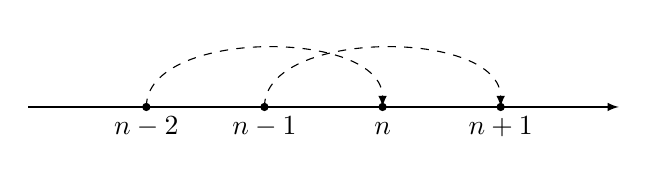
\begin{tikzpicture}[>=latex,x=1.5cm]
			\draw[->] (1,0) -- (6,0);
			\fill (2,0) circle (1.5pt) node [below] {$n-2$};
			\fill (3,0) circle (1.5pt) node [below] {$n-1$};
			\fill (4,0) circle (1.5pt) node [below] {$\phantom{0}n\phantom{0}$};
			\fill (5,0) circle (1.5pt) node [below] {$n+1$};
			\draw[dashed,->] (2,0) .. controls +(0,1) and +(0,1) .. +(2,0);
			\draw[dashed,->] (3,0) .. controls +(0,1) and +(0,1) .. +(2,0);
		\end{tikzpicture}
	\end{center}

	The amplification factor satisfies
	%
	\begin{equation*}
		A^2 - 2 i \kappa \Delta t A -1 =0
	\end{equation*}
	%
	so
	%
	\begin{equation*}
		A_\pm = i \kappa \Delta t \pm \sqrt{ 1 - \kappa^2 \Delta t^2}
	\end{equation*}
	%
	which is second-order accurate.
	%
\end{frame}
%
%%%%%%%%%%%%%%%%%%%%%%%%%%%%%%%%%%%%%%%%%%%%%%%%%%%%%%%%%%%%%%%%%%%%%%
%
%
\begin{frame}
	%
	\frametitle{3TL schemes: Leapfrog}
	%
	There are 2 solutions corresponding to 2 `modes'. If $\kappa \Delta t \rightarrow 0$ then $A_+ \rightarrow 1$ and $A_- \rightarrow -1$. Therefore,
	%
	\begin{align*}
		A_+ &\quad\sim\quad\text{physical mode}\\
		A_- &\quad\sim\quad\text{purely artificial `computational' mode}
	\end{align*}
	%
	\begin{itemize}
		\item If $| \kappa \Delta t | \le 1$, $| A_+ |= |A_-|=1$ so the scheme is stable.\vspace*{2ex}
			%
		\item If $\kappa \Delta t > 1$
			%
			\begin{equation*}
				|A_+ |= \left| i \kappa \Delta t + i \sqrt{\left( \kappa^2 \Delta t^2 - 1 \right)} \right| > |i \kappa \Delta t |> 1
			\end{equation*}
			%
			So the scheme is unstable.\vspace*{2ex}
			%
		\item If $\kappa \Delta t < -1$ then $|A_- |>1$ so the computational mode is unstable.
			%
	\end{itemize}
	%
\end{frame}
%
%%%%%%%%%%%%%%%%%%%%%%%%%%%%%%%%%%%%%%%%%%%%%%%%%%%%%%%%%%%%%%%%%%%%%%
%
%
\begin{frame}
	%
	\frametitle{3TL schemes: Leapfrog}
	%
	The computational mode is easy to analyse in the case $\kappa = 0$:
	%
	\begin{equation*}
		\phi^{n+1} = \phi^{n-1}
	\end{equation*}
	%
	and the roots are $A_+ = 1, A_- = -1$
	%
	\par
	For the initial condition $\phi^0 = C$:
	%
	\begin{equation*}
		\phi^2 = \phi^4 = \phi^6 = \dots = C
	\end{equation*}
	%
	\par
	$\phi^1$ is usually determined by another two-time-level scheme: $\phi^1 = C + \epsilon$ with $\epsilon$ some error. Then
	%
	\begin{equation*}
		\phi(t) = \left\{\,C\,,\,C+\epsilon\,,\,C\,,\,C+\epsilon\,,\,C\,,\,C+\epsilon\,\ldots\,\right\}
	\end{equation*}
	%
	So the error $\epsilon$ stays in the solution.
	%
\end{frame}
%
%%%%%%%%%%%%%%%%%%%%%%%%%%%%%%%%%%%%%%%%%%%%%%%%%%%%%%%%%%%%%%%%%%%%%%
%
%
\begin{frame}
	%
	\frametitle{3TL schemes: Leapfrog}
	%
	The relative phase change of the physical mode of the leapfrog scheme is given by
	%
	\begin{align*}
		R_{\text{leapfrog}} &= \frac{1}{\kappa \Delta t} \arctan \left( \frac{\kappa \Delta t}{\sqrt{ 1 - \kappa^2 \Delta t^2 }} \right) \\
		&\approx 1 + \ft16 \left( \kappa \Delta t \right)^2
	\end{align*}
	%
	So the leapfrog scheme is accelerating.
	%
\end{frame}
%
%%%%%%%%%%%%%%%%%%%%%%%%%%%%%%%%%%%%%%%%%%%%%%%%%%%%%%%%%%%%%%%%%%%%%%
%
\begin{frame}
	%
	\frametitle{3TL schemes: Adams-Bashforth}
	%
	\par
	The trapezium scheme is very attractive (neutral, 2nd order, small phase error), but it is implicit: it requires $F(\phi^{n+1})$ to determine $\phi^{n+1}$.
	%
	\par\vspace*{2ex}
	The Heun scheme attempts to approximate the trapezium scheme by using a forward estimate in the RHS:
	%
	\begin{center}
		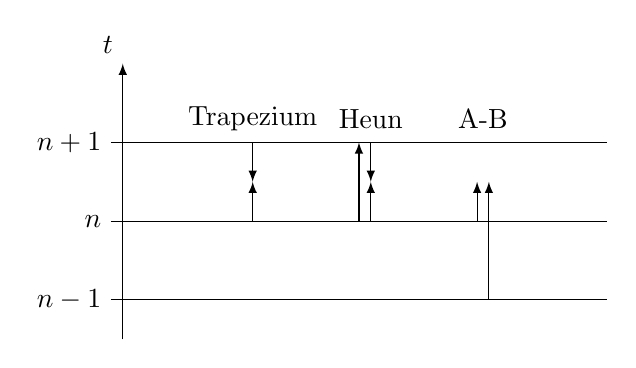
\begin{tikzpicture}[>=latex,x=15mm]
			\draw[->] (0,-1.5) -- (0,2) node[above left] {$t$};
			\draw (-.1,0) node[left] {$n$} -- (4.1,0);
			\draw (-.1,1) node[left] {$n+1$} -- (4.1,1);
			\draw[->] (1.1,0) -- (1.1,.5);
			\draw[->] (1.1,1) -- (1.1,.5);
			\draw (1.1,1.3) node {Trapezium};
			\draw[->] (2,0) -- (2,1);
			\draw[->] (2.1,0) -- (2.1,.5);
			\draw[->] (2.1,1) -- (2.1,.5);
			\draw (2.1,1.3) node {Heun};
		\uncover<2->{%
			\draw (-.1,-1) node[left] {$n-1$} -- (4.1,-1);
			\draw[->] (3,0) -- (3,.5);
			\draw[->] (3.1,-1) -- (3.1,.5);
			\draw (3.05,1.3) node {A-B};%
		}
		\end{tikzpicture}
	\end{center}
	%
	\par
	\uncover<2->{The Adams-Bashforth scheme estimates $F\left(\phi^{n+\ft12}\right)$ by extrapolating from $F\left(\phi^n\right)$ and $F\left(\phi^{n-1}\right)$.}
	%
\end{frame}
%
%%%%%%%%%%%%%%%%%%%%%%%%%%%%%%%%%%%%%%%%%%%%%%%%%%%%%%%%%%%%%%%%%%%%%%
%
%
\begin{frame}
	%
	\frametitle{3TL schemes: Adams-Bashforth}
	%
	The Adams-Bashforth scheme writes:
	%
	\begin{align*}
		F\left(\phi^{n+\ft12}\right)	&=	\ft32 F \left(\phi^n \right) -\ft12 F\left(\phi^{n-1}\right) \\
		\phi^{n+1} &= \phi^n + \Delta t F\left(\phi^{n+\ft12}\right)
	\end{align*}
	%
	For the oscillation equation, the amplification factor satisfies
	%
	\begin{equation*}
		A^2 - \left(1+\ft32 i \kappa \Delta t \right) A + \ft12 i \kappa \Delta t = 0
	\end{equation*}
	%
	with two modes,
	%
	\begin{equation*}
		A_\pm = \ft12 \left[ 1 + \ft32 i \kappa \Delta t\pm \sqrt{1 - \ft94 \left(\kappa \Delta t \right)^2 + i \kappa \Delta t }\right]
	\end{equation*}
	%
\end{frame}
%
%%%%%%%%%%%%%%%%%%%%%%%%%%%%%%%%%%%%%%%%%%%%%%%%%%%%%%%%%%%%%%%%%%%%%%
%
%
\begin{frame}
	%
	\frametitle{3TL schemes: Adams-Bashforth}
	%
	For good temporal resolution $\kappa\Delta\leq1$,
	%
	\begin{align*}
		|A_+|_\text{A-B2} &\approx 1 + \ft14 \left( \kappa \Delta t \right)^4	\\
		|A_-|_\text{A-B2} &\approx \ft12 \kappa \Delta t\\
		R_\text{A-B2} &\approx 1 + \ft{5}{12} \left( \kappa \Delta t \right)^2
	\end{align*}
	%
	\par\bigskip
	In NWP application we want strict stability, so this weak instability makes Adams-Bashforth unattractive.
	%
	\par\medskip
	In contrast, the leapfrog mode contains the artificial computational mode. However, this mode can be controlled by a Robert-Asselin filter.
	%
\end{frame}
%
%%%%%%%%%%%%%%%%%%%%%%%%%%%%%%%%%%%%%%%%%%%%%%%%%%%%%%%%%%%%%%%%%%%%%%
%
\begin{frame}
	%
	\frametitle{The Robert-Asselin filter}
	%
	We modify the leapfrog-scheme by adding a filter step:
	%
	\begin{align*}
		\phi^{n+1} & = \overline{\phi^{n-1}} + 2 \Delta t F(\phi^n )	&&\text{normal leapfrog}\\
		\overline{\phi^n} & = \phi^n + \gamma \left(\overline{\phi^{n-1}} - 2 \phi^n + \phi^{n+1}\right)&&\text{apply filter}
	\end{align*}
	%
	where typically $\gamma = 0.06$ in meteorological models.
	%
	\uncover<2->{
	\par\medskip
	The term $\overline{\phi^{n-1}} - 2 \phi^n + \phi^{n+1}$ can be interpreted as a temporal filter that damps the high frequencies (esp. the $2\Delta t$-mode): if $\overline{\phi^{n-1}}>\phi^n$ and $\phi^{n+1}>\phi^n$, then $\overline{\phi^n}$ will be increased:
	%
	\begin{center}
		\begin{tikzpicture}[>=latex,y=5mm]
			\draw (0,2) node [above left] {$\overline{\phi^{n-1}}$} -- 
				(2,0) node [below] {$\phi^{n}$} -- 
				(4,3) node [above right] {$\phi^{n+1}$};
			\draw[->] (2,0) -- (2,1) node [above]  {$\overline{\phi^{n}}$};
			\fill (0,2) circle (1.5pt) (2,0) circle (1.5pt) (4,3) circle (1.5pt);
		\end{tikzpicture}
	\end{center}
	}
\end{frame}
%
%%%%%%%%%%%%%%%%%%%%%%%%%%%%%%%%%%%%%%%%%%%%%%%%%%%%%%%%%%%%%%%%%%%%%%
%
%
\begin{frame}
	%
	\frametitle{The Robert-Asselin filter}
	%
	Amplification of Asselin-leapfrog:
	%
	\begin{equation*}
		A_\pm = \gamma + i \kappa \Delta t \pm \sqrt{\left( 1 - \gamma \right)^2 - \kappa^2 \Delta t^2}
	\end{equation*}
	%
	For small $\kappa \Delta t$, 
	%
	\begin{align*}
		A_+ & \approx 1 + i \kappa \Delta t -\frac{(\kappa \Delta t)^2}{2 (1-\gamma)}	\\
		A_-	&	\approx -1+2\gamma+i\kappa\Delta t+\frac{(\kappa \Delta t)^2}{2 (1-\gamma)}
	\end{align*}
	%
	while expansion of the exact solution is:
	%
	\begin{equation*}
		A_e = e^{i \kappa \Delta t} = 1 +i \kappa \Delta t - \ft12 \left( \kappa \Delta t \right)^2- i \ft16 \left( \kappa \Delta t \right)^3 + O[(\kappa \Delta t)^4 ]
	\end{equation*}
	%
	So the Robert-Asselin filter degrades the accuracy of the scheme from 2nd order to 1st order.
	%
\end{frame}
%
%%%%%%%%%%%%%%%%%%%%%%%%%%%%%%%%%%%%%%%%%%%%%%%%%%%%%%%%%%%%%%%%%%%%%%
%
%
\begin{frame}
	%
	\frametitle{The Robert-Asselin filter}
	%
	The modulus of the amplification factor becomes:
	%
	\begin{align*}
		|A_+| &\approx 1 - \frac{\gamma}{2 (1 - \gamma)} (\kappa \Delta t)^2 \\
		|A_-| &\approx (1-2\gamma) + \frac{\gamma}{2 - 6 \gamma + 4 \gamma^2} (\kappa \Delta t)^2
	\end{align*}
	%
	Note that the computational mode is (slightly) damped.
	%
	\par\vspace*{2ex}
	The relative phase change becomes:
	%
	\begin{equation*}
		R_+ \approx 1 + \frac{1+2\gamma}{6 (1-\gamma)} (\kappa \Delta t)^2
	\end{equation*}
	%
\end{frame}
%
%%%%%%%%%%%%%%%%%%%%%%%%%%%%%%%%%%%%%%%%%%%%%%%%%%%%%%%%%%%%%%%%%%%%%%
%
\begin{frame}
	%
	\frametitle{3-timelevel schemes}
	%
	Exercise: section 3 of the Jupyter notebook \texttt{time\_discretization.ipynb}
	%
\end{frame}
%
%%%%%%%%%%%%%%%%%%%%%%%%%%%%%%%%%%%%%%%%%%%%%%%%%%%%%%%%%%%%%%%%%%%%%%
%
\begin{frame}
	%
	\frametitle{Summary}
	%
	\begin{itemize}
		\item We work on the \emph{oscillation equation}, to focus on the time differencing aspect\vspace*{3ex}
		\item A scheme is characterized by
			\begin{itemize}
				\item amplitude: amplifying, neutral or damping
				\item relative phase change: accelerating or decelerating
				\item explicitness or implicitness
				\item order of accuracy\vspace*{3ex}
			\end{itemize}
		\item Concrete examples:
			\begin{itemize}
				\item Two time-level schemes: forward, backward, \textbf{trapezium}
				\item Multistage schemes: Heun, Matsuno, \textbf{Runge-Kutta-4}
				\item Three time-level schemes: \textbf{leapfrog} and Adams-Bashforth\\
					{\hspace*{5mm}$\Rightarrow$ computational mode, filter}\vspace*{3ex}
			\end{itemize}
		\item There is no `best' scheme: every scheme has disadvantages.\vspace*{3ex}
		\item What matters is methodology!
	\end{itemize}
	%
\end{frame}
%
%%%%%%%%%%%%%%%%%%%%%%%%%%%%%%%%%%%%%%%%%%%%%%%%%%%%%%%%%%%%%%%%%%%%%%
%
\end{document}
